% This file is part of \tc\   project.
% Copyright 2015 the authors.

% style notes
% - \,percent not \%

\documentclass[14pt, preprint2]{aastex6}
\usepackage{bm, graphicx, subfigure, amsmath, morefloats}


%\documentclass[12pt, preprint]{aastex}
%\usepackage{bm, graphicx, subfigure, amsmath, morefloats}
\usepackage{longtable}
% words
\newcommand{\project}[1]{\textsl{#1}}
\newcommand{\thecannon}{\project{The~Cannon}} 
\newcommand{\tc}{\project{The~Cannon}} 
\newcommand{\apogee}{\project{\textsc{apogee}}}
\newcommand{\apokasc}{\project{\textsc{apokasc}}}
\newcommand{\aspcap}{\project{\textsc{aspcap}}}
\newcommand{\corot}{\project{Corot}}
\newcommand{\kepler}{\project{Kepler}}
\newcommand{\gaia}{\project{Gaia}}
\newcommand{\gaiaeso}{\project{Gaia--\textsc{eso}}}
\newcommand{\galah}{\project{\textsc{galah}}}
\newcommand{\most}{\project{\textsc{most}}}
\newcommand{\code}[1]{\texttt{#1}}
\newcommand{\documentname}{\textsl{Article}}

\newcommand{\teff}{\mbox{$\rm T_{eff}$}}
\newcommand{\kms}{\mbox{$\rm kms^{-1}$}}
\newcommand{\feh}{\mbox{$\rm [Fe/H]$}}
\newcommand{\xfe}{\mbox{$\rm [X/Fe]$}}
\newcommand{\alphafe}{\mbox{$\rm [\alpha/Fe]$}}
\newcommand{\mh}{\mbox{$\rm [M/H]$}}
\newcommand{\logg}{\mbox{$\rm \log g$}}
\newcommand{\noise}{\sigma_{n\lambda}}
\newcommand{\scatter}{s_{\lambda}}
\newcommand{\pix}{\mathrm{pix}}
\newcommand{\rfn}{\mathrm{ref}}
\newcommand{\rgc}{\mbox{$\rm R_{GC}$}}
\newcommand{\rgal}{\mbox{$\rm R_{GAL}$}}
\newcommand{\vgal}{\mbox{$\rm V_{GAL}$}}

% math and symbol macros
\newcommand{\set}[1]{\bm{#1}}
\newcommand{\starlabel}{\ell}
\newcommand{\starlabelvec}{\set{\starlabel}}
\newcommand{\mean}[1]{\overline{#1}}
\newcommand{\given}{\,|\,}

% math
\newcommand{\numax}{$\nu_{\max}$}
\newcommand{\deltanu}{$\Delta\nu$}
\bibliographystyle{apj}

\keywords{
%Evidence that NGC6791 is disrupting
---
methods: data analysis
---
methods: statistical
---
stars: evolution
---
stars: fundamental parameters
---
techniques: spectroscopic
}

\begin{document}

%-- canonical siblings


%\title{Chemical Pairs I: assessment of the homogenity of open clusters}
%\title{Chemical nearest neighbours: The precision of the measurements of APOGEE spectra}
%\title{Chemical nearest neighbours I: open clusters are not nearest neigbours in chemical space}
\title{Precision Abundances for seven open clusters in APOGEE  }
\author{M.~Ness\altaffilmark{1},
        H-W.~Rix\altaffilmark{1}, 
        D.~W.~Hogg\altaffilmark{1,2,3},
         A.R. Casey, M. Fouesneau, Y-S. Ting (order TBD)}
        % paper title 2: constraints on the effect of radial migration in the Milky Way at a median timescale of 3 Gyr - AMY
        % observational constraints 
        % radial migration is an insignificant affect on the orbits of APOGEE red clump stars. 


\altaffiltext{1}{Max-Planck-Institut f\"ur Astronomie, K\"onigstuhl 17, D-69117 Heidelberg, Germany}
\altaffiltext{2}{Center for Cosmology and Particle Physics, Department of Phyics, New York University, 4 Washington Pl., room 424, New York, NY 10003, USA}
\altaffiltext{3}{Center for Data Science, New York University, 726 Broadway, 7th Floor, New York, NY 10003, USA}
\altaffiltext{4}{UCLAN}
\email{ness@mpia.de}

\begin{abstract} 

We report 20 precision abundances for 92 red giant stars in 8 targeted open clusters in the \apogee\ dataset measured by \tc. To obtain our high precision results, we had to make modifications to \tc\ to deal with fiber LSF variations that introduce systematic abundance offsets. We measure the abundance variations in the clusters, which are general proxies for single stellar birth sites, in order to understand how homogeneous these birth sites are -- and how similar two sibling stars in the \apogee\ dataset are expected to be. We measure Fe, C, N, O, Na, Mg, Al, Si, S, K, Ca, Ti, V, Mn, Ni, P, Cr, Co, Cu, Rb for stars in NGC7789, NGC6819, NGC6791, NGC2420, NGC2158, NGC188 and M67. We find the measured scatter in [X/Fe] of the clusters in these 20 elements to be typically 0.01 $-$ 0.07 dex. We construct a model of our cluster data given the abundance errors for each cluster at the signal to noise (SNR) of each observation and conclude that open clusters have no \textit{intrinsic} scatter in the alpha, light and iron-peak elements that we measure. However, the clusters NGC2420, M67, NGC2158 and NGC6791 have a small (0.01 - 0.03 dex) intrinsic scatter in \feh. From examining the distribution of nearest chemical neighbours both between and among clusters, we conclude that if two stars in the \apogee\ dataset have a $\chi^2_{red}$ $>$ 2.8,  as determined from the 20 elements measured by \apogee, then they are likely to be not born together.  
\end{abstract}

\section{Introduction}

There now exists a plethora of spectroscopic data across the disk of the Milky Way for which large numbers of abundances have been measured. This data is being delivered by current surveys including Gaia-ESO \citep{gilmore2012}, APOGEE \citep{Majewski2015} and GALAH \citep{Freeman2012, deSilva2015} and there are numerous future spectroscopic surveys being planned e.g. 4MOST \citep{deJong2015}, MOONS \citep{C2012}, WEAVE \citep{D2012}. Large volumes of data, combined with new techniques to optimally exploit the data and deliver high precision stellar abundances (e.g. The Cannon; \citep{Ness2015, Casey2016} enable us to examine the distribution in abundance space of the stars in the Milky Way disk and halo and to pursue chemical tagging (e.g. Hogg et al., 2016), where by coherent structures are identified using similarity in high-dimensional abundance space only.  

% gaia release: only 2500 open clusters known in the MW - around the Sun and expect about 100,000 clusters
% clusters are difficult to find: can be found via motions moving together combined with abundances: we use pairs as beacons. 

%Studies using the abundances in large surveys have focused in large part on using only one or two elements mapped across the galaxy (e.g. Gilmore's paper) and outliers (Shiavon, Martel) or specific objects of interest like open and globular clusters (list here). The data is also hard to interpret in the current theoretical framework: even the \alphafe\ distribution across $(R,z)$ is not straightforward to tie back to theoretical expectations of chemical enrichment although offers insight into radial migration (e.g. Hayden, Nidiver).  Ultimately, the multitude of abundances for large numbers of stars across a large radial extent of the disk is difficult to map to interpretable results so we need metrics to pursue this, one of which is chemical tagging, another of which as we propose here is using nearest neighbour pairs. To implement either metric, we must first understand the distribution in abudances of those stars that are known to be born together, of which the disk is expected to be comprised of dissolved groups of. 
% Part of this is that the theoretical expectations are divergent from the data including for looking only at the \alphafe\ distribution only 
%
%We make a model to determine the intrinsic dispersion of these clusters, given our measurements and our errors.  The intra-cluster similarity we find between two of the clusters at similar [Fe/H] highlights the likely largest challenge for chemical tagging, as it is currently envisioned, which is not that open clusters may not be entirely homogeneous (e.g. Asplund's recent paper) but that clusters may have extremely similar abundance signatures and unable to be separated using chemistry alone. % of the full disk so can set a metric of when two stars are not born in the same molecular cloud. % stars of a common birth origin  and to describe the dynamical and spatial properties of stars that are most to least chemically similar, conditioned on expectations from properties of open clusters

%The inter-cluster and intra-cluster dispersion sets our expectation of abundance similarity of stellar siblings, which is relevant to chemical tagging, which is a discrete and specific approach for reconstructing the building blocks of the disk in order to understand its formation history. We conclude by discussing a more general approach: we propose a pair metric of stars with similar abundances.  That is, examining the spatial and dynamical distribution of nearest neighbours in abundance space, where these nearest neighbours need \textit{not} be stellar siblings. Examining pairs of stars with extreme similarity in abundance space and mapping their orbital distributions, which coming years of Gaia data will allow, will enable us to understand numerous properties of the disk. This includes placing constraints on how well the star-forming gas of the Milky Way disk was mixed (as revealed only in multi-element abundance space this can not be tested from the \alphafe\ alone) and if the disk formed irregularly or else in concentric rings, as it grew from the inside out (e.g. Ness et al., 2016). This can be achieved without the constraint that the nearest-neighbour pairs be stellar siblings. We demonstrate that for  the 20,000 red clump sample of \apogee, the pair metric does return pairs that are true stellar siblings from known clusters, including a previously unclassified member of the cluster NGC188, lying outside the nominal cluster radius (Harris et al., 2006). 

Our aim is to understand the current day chemical abundance distribution of stars in the the Milky Way disk disk and trace back its assembly history. One discrete way to pursue this is to identify stars of common birth sites via their abundance signatures, so called chemical tagging \citep{freeman2002}. To do this, we need to first know what the spread is in the abundance measurements of stars that are known to be born together.  The dispersion that we measure in groups of stars that are born together, or clusters, is a combination of the intrinsic dispersion of the cluster and the measurement precision we can achieve. Measuring this total dispersion for the clusters is necessary to calibrate our expectations in assessing the chemical abundance distribution and dimensionality of the Milky Way disk and for being able to determine when stars are likely to be \textit{not} born together. 

Recently, \citet{Bovy2016} used a data-driven methodology to demonstrate that three open clusters in \apogee; M67, NGC6819 and NGC2410 are chemically homogeneous. Bovy (2016) used the stellar spectra directly, showing that after removing temperature trends, the cluster spectra form one-dimensional sequences. This novel approach was motivated by the difficulties in obtaining consistent high precision stellar abundances and it is optimal to achieve very high precision limits on the intrinsic cluster abundance dispersions, and so assess homogeneity of a single birth site itself. However, the limitation in such a method is that it does not return an absolute abundance measurement. Our aim is to to address the problem of providing consistent high-precision abundances.  Absolute measurements are needed to measure the chemical diversity, distribution and, conditioned on expectations of the properties of open clusters, the chemical dimensionality of the disk: that is, measuring how many discrete building blocks it is comprised of.  The high precision abundance measurements for the open cluster stars in \apogee\ and their inter-cluster abundance dispersions, which we determine, provides the calibration or expectation properties for stars that are born together and also not born together. With our modifications to the Cannon and carefully selected high-fidelity training set, we achieve near the precision of Bovy et al, (2016) for many elements, but report absolute abundance measurements, for 90 open cluster stars. 

The key ingredients for delivering our high precision measurements are (i) our modifications both \tc\ and to the training set abundances to correct for the abundance variation across fiber number, due to the varying Line Spread Function (LSF) across the APOGEE plate and (ii) selecting a high fidelity training set from ASPCAP; we used 5000 high signal to noise stars and trained our data driven model on three stellar parameters, \teff, \logg\ and \feh\ and 19 [X/Fe] individual abundances from DR13 \citep{Holtzman2015}.   In Section 3 we present our training set and in Section 5 our cross-validation results, which shows the highest precision we can measure for each of our parameters and abundances (with the signal to noise dependent precision reported in the Abstract. We discuss the problem of LSF variation and our correction and modification to The Cannon to cope with this in Section 4 and in Section 5
we report the abundance trends for each of the individual clusters which we discuss in Section 6, determining the intrinsic spread in each element using our cluster model and characterising the inter and intra-cluster stellar similarity using nearest neighbour chemical pairs.  


\section{Method}

We used \tc\ to deliver our high precision abundances, using the quadratic model implementation outlined in \citet{Ness2015}, but train on many labels similarly to \citet{Casey2016}. We also implemented modifications to \tc\ to incorporate the impact of the varying LSF on the spectra and the subsequent \aspcap\ DR13 labels, which we found to have minor systematic dependencies on the LSF (see Section 4).  We measured the LSF for each star in both our training and test set of stars, and included this LSF value as a single additional data point, which is then handled similarly to the flux of the star in \tc. We train on 23 labels in total: 3 stellar parameters, of \teff, \logg\ and \feh\ and 19 abundances that were released in DR13 as well as the LSF.  The LSF variations are already imprinted onto the labels we train on, and the approach we take to include the LSF in our Cannon model and to also make corrections to our training data for the LSF variation is a consequence of this. To properly and optimally correct for the variation in the LSF would require a full modeling of the LSF for each star when deriving the stellar abundance and individual element labels themselves.

\section{The \apogee\ Data}

We used the \apogee\ spectra and stellar parameter and abundances from the SDSS-IV public data release DR13 (Johnson et al., 2016, in prep.). We performed our own signal-to-noise independent continuum normalization on the aspcapstar files, similarly to \citet{Ness2015}, by fitting a second order polynomial to pixels identified with weak parameter dependences. For the new DR13 data we selected again around 5\% of the pixels using a criteria of 0.985 $>$ flux $>$ 1.025 and ($|\theta_{Teff}|$, $|\theta_{logg}|$, $|\theta_{[Fe/H]}|$) $<$  (0.005,0.005,0.005). 

\subsection{Training Data} 

We constructed a training set of data comprised of 5000 stars that span the chemical space of the stars of the Milky Way disk and inclusive in this, our test set of stars of red giant open cluster members.  For our training labels we used the DR13-corrected labels with small additional corrections for the LSF dependence (see section 4). We selected high SNR stars for our training set (SNR $>$ 200) and took care to remove highly anomalous abundance measurements. We also excluded all stars with any bad flag set.  Our training data spans the following range in stellar parameters:\\
\teff\ = 3650 $-$ 5760 K  \\
\logg\ = 0.45 $-$ 3.95 dex \\
\feh\ = --1.7 $-$ 0.36 dex \\

% took care not to 5000 stars in training set 
\subsection{Test Data} 

Our test data are the 97 stars in the open clusters, where our membership is taken from the cross over between those identified by Meszaros et al., (2012) and those in the \apogee\ calibration file table \footnote{cal$\_$dr13.fits available at sdss.org}. For NGC2420 we took an additional 3 stars to those identified in \citet{Meszaros2013}  which were identified (and studied) by \citet{Souto2016}
% as well as  an additional member for NGC188 which we identified using the nearest neighbour approach described in Section 6.3 when determining nearest neighbours for the red clump sample of \citet{Bovy2015}

\section{Modifications to \tc\ to address LSF variation}

Removing systematics that bias the abundance measurements of stars of different spectral types presents one of the most significant practical challenges to consistent and precise abundance measurements. Abundance trends with temperature and surface gravity are dealt with in \apogee\ via a post-calibration, taking out the trends measured from a set of open and globular cluster stars in \apogee\ and \logg\ calibrations using asteroseismic targets with very precise \logg\ values derived from the asteroseismic parameters. A more subtle systematic signature that we found is mapped onto the abundances is fiber number, which is due to the variation of the line spread function across the observing plate and potentially signatures of nonuniform characteristics of the electronics, such as the persistence, which affects only part of the chip from which the spectra is read out (up to fiber number $\approx$ 50 at the lowest values of LSF). 

The relationship between the LSF and the measured abundances is shown in Figure \ref{fig:rclsf}. This Figure shows the mean DR13 abundances of our training set of stars,  as a function of the LSF for the stars, measured from the apStarLSF files provided by \apogee. For mapping the overall trends of abundances across the disk these trends are not significant and will not affect global inferences of example the abundance trends based on the measurements across $(R,z)$, which are on average inclusive of all fiber numbers independent of position on the sky (except for targeted co-natal groups like streams and open and globular clusters). However, these trends are extremely important to remove when deriving the most precise abundances possible and it is necessary to remove these trends to use the abundances in concert to examine chemical similarity. For example, in measuring a distance in abundance space metric between stars (section 6), if there is a systematic dependence on the mean measurement and dispersion of that measurement as a function of LSF, then stars that have the same fiber number are found as preferential nearest chemical neighbours, which is the case using the \aspcap-scale abundances. We also note that the absolute abundance spreads of the clusters with low fiber numbers, which equates to the lowest LSF (e.g. NGC2158, NGC6791, M67) are higher than those with high fiber number,  particularly for problematic elements such as Cu, the mean abundance of which  changes very quickly with LSF or fiber number at the lowest LSF values, which is equivalent to the lowest fiber numbers. 

For our training data, we correct for these systematic biases for each element show in Figure \ref{fig:rclsf} by fitting a 5$^{th}$ order polynomial to the mean trend of each element and adjusting each element by the offset given by the fit, so as the mean of every abundance as a function of LSF is then 0. These values become our input LSF-corrected training labels.  For most elements this correction is very small and for some it is negligible, but for elements like Cu it can be as high as 0.2 dex for the lowest LSF value (see Figure \ref{fig:training}).

%We therefore input as our training labels our own LSF-corrected versions of \aspcap's corrected (for temperature and logg systematics) DR13 values. 
% /Users/ness/new_laptop/Apogee_DR12_play/DR13_calibrated
%run -i makelist_LSFscatter_H_paper.py
\begin{figure*}[h!]
%\centering
%\includegraphics[scale=0.6]{/Users/ness/new_laptop/Apogee_DR12_play/DR13_calibrated/training_input.pdf} 
\includegraphics[scale=0.6]{training_input.pdf} 
  \caption{The mean measurements of the \aspcap\ DR13-corrected labels as a function of measured LSF for the 5000 stars used for the training set. The dispersion around the mean measurement is shown in the gray shaded region. The largest difference in the mean and the dispersion around the mean is written at the top of each panel. We correct for these offsets to produce LSF-corrected labels that we use for training for \tc. For many elements this correction is negligible, for some, like Cu, this is significant.  }
\label{fig:training}
\end{figure*}

%key to remove systematics - put in plot of red clump apogee

%for highest precision found a modest training set worked best, used 536 stars covering the metallicity range of the red clump only, spanning Teff X -- Y , logg X -- Y and [Fe/H] == X -- Y 
% need to discuss that use entire region: want highest precision - legit thing to do . 

\section{Results}

\subsection{Cross validation of training set} 

%run -i makeself.py

\begin{figure*}[h!]
%\centering
%\includegraphics[scale=0.45]{/Users/ness/new_laptop/Apogee_elements/redclump_chi2/training/crossval_5026.pdf} 
\includegraphics[scale=0.45]{crossval_5026.pdf} 
  \caption{Take 10-percent out cross validation test. All elements are with respect to Fe except for Fe, which is respect to H. The x-axis shows our input labels and the y-axis shows \tc's output labels. }
\label{fig:cross}
\end{figure*}

The precision with which we can determine our labels is measured using the cross-validation test on the training set, similarly to \citet{Ness2015, Ho2016, Casey2016}. Our cross-validation performance, for our leave-10-percent-out test is shown in Figure \ref{fig:cross}. The stars in this Figure have all been excluded from the training set. The model that is constructed when the stars are excluded, in 10 $\times$ 10-percent subsets is the model that is used to derive their plotted labels. The x-axis shows the input training labels and the y-axis shows \tc's best fit labels. We are able to recover the labels high precision, for example, for the stellar parameters the precision is approximately $<$ 45 K in \teff, $<$ 0.1 dex in logg and $<$ 0.02 dex in \feh and for individual abundances, the precision is on the order of 0.02 -- 0.12 dex, depending on the element. 

\subsection{Open Cluster Results} 

Our model fit to the data is excellent and we show a typical star from our test data, from the cluster NGC6791 in Figure \ref{fig:typical}. A broad, 300 Angstrom span of the spectra of this star (in black) and model (in cyan) is shown in the top panel of the Figure. The scatter of the model itself is shown in the panel directly underneath, for the same 300 Angstrom spectral region. The small scatter demonstrates that the model is a good overall fit to the training data -- and thus the test data, presuming the training data is representative of the label space of the test data test data which is one of our primary assumptions (see the Discussion in Ness et al., 2015). Narrow wavelength regions ($\approx$ 8 Angstroms )are also shown Figure \ref{fig:typical}, to demonstrate the goodness of fit of the model around a number of individual element absorption features. For our model and derivation of labels, we do not restrict the pixels that \tc\ uses to deliver the abundance information; indeed the cross validation demonstrates that it learns where the information about each element is derived from in the spectra. This freedom does however enable \tc\ to learn about a given element using correlations of lines other than the specific element being derived: this is the optimal approach for high precision measurements of our 20 elements given our training data, and we expand on this point in the Abstract: with masking implemented to use only particular regions of the spectra to constrain the model to only learn about abundance X using strictly the absorption features X, some of the more poorly measured elements are not able to be well reproduced in cross-validation, thus we have fewer elements that can be measured if we restrict our wavelength regions. That the cross validation demonstrates that we can determine the individual abundances without restricting the wavelengths used indicates that \tc\ learns where the information in the spectra is about each element, but that this may include correlations from other lines than the abundance being measured; essentially, this mathematically works and our goodness of fit, $\chi^2$ metric can indicate any results which are unreliable. 

From the goodness of fit $\chi^2$ metric which we determined for each star, we excluded 7 stars, all from the cluster NGC6917 and 3 from M71, with a $\chi{_red}^2$ $>$ 3. For our analysis of the cluster data, we do not exclude cluster stars with relatively low SNR measurements (SNR $<$ 100), but use the SNR dependent error to estimate the scaled precision at low SNR (see the Appendix). Our cluster stars have a reported SNR from 60 to 1000. Our errors for each star are the quadratic sum of the signal-to-noise scaled cross-validation errors, plus the formal errors that are returned by the optimizer at test time running \tc. 

Figures \ref{c1} to \ref{c7} show the cluster individual abundances plotted coloured by \teff with their corresponding error bars. Typical absolute dispersion measurements for the clusters range from 0.01 -- 0.1 depending on the element.  The cyan points in the background are the training data. The DR13 input abundance labels that we adopt for training are corrected for systematic variations with temperature, except for C and N, which are known to have astrophysical variations along the giant branch. For the open clusters, we note that the coolest stars do seem to have the highest measurements of [N/Fe], within a cluster. 

We report the measured mean and dispersion for our 90 open cluster stars in Table 1 as well as the \aspcap\ results (where available) and provide the measurements for each star as well as their 2MASS ID's in our online table. Our results compare very well to the \aspcap\ results, but using \tc, we obtain far higher precision and so report dispersions on the order of 20-50\% lower than \aspcap, in most cases. We are concerned with precision and not accuracy and there is a discussion in \citet{Holtzman2016} regarding the scale of the open clusters with respect to the literature. Overall, we note there is a large literature dispersion in individual element measurements from high resolution spectroscopy (e.g. see Table 3 of Souto et al., 2016 for NGC2420). 


\begin{table*}[!h]
\centering
\tiny
\begin{tabular}{ | p{0.04\textwidth} | c| c | c | c | c | c | c | c | }
\hline
\multicolumn{1}{|c|}{Element}& \multicolumn{2}{|c|}{NGC7789 (5 stars)} & \multicolumn{2}{|c|}{NGC6819 (27 stars)}  & \multicolumn{2}{|c|}{NGC6791 (23 stars)} & \multicolumn{2}{|c|}{ NGC188 (3 stars)} \\
\hline
%Element & NGC7789 (5 stars) & -- & -- & NGC6819 (27 stars) & NGC6791 (23 stars)& -- & NGC188 (3 stars) & -- \\
 &  ASPCAP & The Cannon & APSCAP & The Cannon & ASPCAP & The Cannon & ASPCAP & The Cannon \\
 \hline
Fe &  -0.05 $\pm$ 0.05  & -0.04 $\pm$ 0.07 &  0.04 $\pm$ 0.04   & 0.03 $\pm$ 0.04  &  0.29 $\pm$ 0.05  & 0.21 $\pm$ 0.08 &   0.05 $\pm$ 0.02 & 0.05 $\pm$ 0.01   \\
C & -0.08 $\pm$ 0.07  & -0.08 $\pm$ 0.02' & -0.05 $\pm$ 0.09 & -0.04 $\pm$ 0.04 & 0.18 $\pm$ 0.1 &0.18 $\pm$ 0.06 & 0.0 $\pm$ 0.05 & 0.0 $\pm$ 0.04 \\
N &  0.37 $\pm$ 0.07 & 0.36 $\pm$ 0.03 & 0.33 $\pm$ 0.08 & 0.33 $\pm$ 0.07 & 0.32 $\pm$ 0.07 & 0.29 $\pm$ 0.07 &  0.36 $\pm$ 0.17 & 0.34 $\pm$ 0.14 \\
O & 0.01 $\pm$ 0.08 & 0.02 $\pm$ 0.02 &  0.01 $\pm$ 0.06  & -0.01 $\pm$ 0.03 & 0.1 $\pm$ 0.07 & 0.12 $\pm$ 0.05 & 0.07 $\pm$ 0.03  & 0.03 $\pm$ 0.01 \\
Na & -0.03 $\pm$ 0.0XXX & -0.13 $\pm$ 0.05 &  0.01 $\pm$ 0.06  & 0.02 $\pm$ 0.04 & 0.09 $\pm$ 0.08 & 0.15 $\pm$ 0.09 &  0.08 $\pm$ 0.02 & -0.12 $\pm$ 0.07 \\
Mg  & -0.02 $\pm$ 0.05 & -0.02 $\pm$ 0.0 &   -0.0 $\pm$ 0.04 & 0.01 $\pm$ 0.01 & 0.1 $\pm$ 0.06 & 0.11 $\pm$ 0.04 &  0.03 $\pm$ 0.05 & 0.04 $\pm$ 0.02 \\
Al  & -0.07 $\pm$ 0.06 & -0.04 $\pm$ 0.0  & -0.02 $\pm$ 0.05 & -0.02 $\pm$ 0.04- & 0.1 $\pm$ 0.11  & 0.01 $\pm$ 0.07 & 0.03 $\pm$ 0.03  & 0.02 $\pm$ 0.02 \\
Si & -0.01 $\pm$ 0.08 & -0.03 $\pm$ 0.01 &  0.02 $\pm$ 0.05 & 0.01 $\pm$ 0.04 & 0.14 $\pm$ 0.06  & 0.0 $\pm$ 0.03 & 0.04 $\pm$ 0.01  & 0.03 $\pm$ 0.01  \\
S & -0.02 $\pm$ 0.03 &  0.04 $\pm$ 0.06 &  0.01 $\pm$ 0.05 & -0.01 $\pm$ 0.07  & 0.02 $\pm$ 0.06 & -0.06 $\pm$ 0.06 & 0.0 $\pm$ 0.05   &  0.04 $\pm$ 0.04 \\
K & 0.11$\pm$ 0.1 & -0.01 $\pm$ 0.03 & -0.01 $\pm$ 0.1 & -0.01 $\pm$ 0.03 &  0.09 $\pm$ 0.15  & 0.03 $\pm$ 0.04 & -0.04 $\pm$ 0.05  & 0.02 $\pm$ 0.01  \\
Ca & -0.01$\pm$ 0.08 & -0.01 $\pm$ 0.03 & -0.01 $\pm$ 0.05  & 0.0 $\pm$ 0.01 & 0.02 $\pm$ 0.08 & 0.05 $\pm$ 0.04 &  -0.03 $\pm$ 0.07 & -0.04 $\pm$ 0.02 \\
Ti & -0.01$\pm$ 0.06 & -0.04 $\pm$ 0.02 & 0.01 $\pm$ 0.04  & 0.0 $\pm$ 0.03 & 0.02 $\pm$ 0.09 & 0.08 $\pm$ 0.05 &  -0.03 $\pm$ 0.03 & 0.03 $\pm$ 0.07 \\
V & -0.01$\pm$ 0.1 &  -0.01 $\pm$ 0.02 & 0.01 $\pm$ 0.06 & 0.03 $\pm$ 0.06 & 0.07 $\pm$ 0.14 & 0.09 $\pm$ 0.07 & 0.0 $\pm$ 0.05  & 0.04 $\pm$ 0.04 \\
Mn & -0.02 $\pm$ 0.06 & -0.02 $\pm$ 0.01  &  0.0 $\pm$ 0.04 & 0.0 $\pm$ 0.01 & 0.02 $\pm$ 0.09 & 0.06 $\pm$ 0.02 & 0.01 $\pm$ 0.06  & 0.03 $\pm$ 0.03 \\
Ni & -0.02 $\pm$ 0.06 & -0.02 $\pm$ 0.02  &  0.01 $\pm$ 0.04 & 0.01 $\pm$ 0.01 & 0.03 $\pm$ 0.07 & 0.04 $\pm$ 0.02 & 0.03 $\pm$ 0.03  & 0.02 $\pm$ 0.02 \\
P & -0.06 $\pm$ 0.07 &  -0.14 $\pm$ 0.06  & -0.05 $\pm$ 0.15 & -0.12 $\pm$ 0.11 & 0.06 $\pm$ 0.11 & 0.01 $\pm$ 0.11 & 0.08 $\pm$ 0.03  & -0.02 $\pm$ 0.08 \\
Cr & 0.02 $\pm$ 0.08 &  0.03 $\pm$ 0.03 &  0.01 $\pm$ 0.05 & 0.02 $\pm$ 0.02 & -0.08 $\pm$ 0.08 &0.02 $\pm$ 0.03 & -0.04 $\pm$ 0.08  &  0.02 $\pm$ 0.01 \\
Co & -0.01$\pm$ 0.11 & 0.03 $\pm$ 0.05 &  0.04 $\pm$ 0.07 & 0.06 $\pm$ 0.04 & 0.17 $\pm$ 0.07 & 0.16 $\pm$ 0.06 &  0.15 $\pm$ 0.07 &  0.11 $\pm$ 0.04 \\
Cu &  0.0 $\pm$ 0.1 & -0.01 $\pm$ 0.02 & 0.1 $\pm$ 0.08 & 0.17 $\pm$ 0.05 & XXX $\pm$ 0.0 & 0.05 $\pm$ 0.12 &  -0.03 $\pm$ 0.11 & -0.06 $\pm$ 0.06 \\
Rb & 0.05 $\pm$ 0.05 & 0.04 $\pm$ 0.01  &  0.01 $\pm$ 0.07 & 0.06 $\pm$ 0.04 & 0.01 $\pm$ 0.11 & 0.04 $\pm$ 0.12 & 0.06 $\pm$ 0.02  & 0.09 $\pm$ 0.01 \\
 \hline
\multicolumn{1}{|c|}{Element}& \multicolumn{2}{|c|}{ NGC2420 (12 stars)} & \multicolumn{2}{|c|}{NGC2158 (7 stars)}  & \multicolumn{2}{|c|}{M67 (19 stars)} & \multicolumn{2}{|c|}{M71 (2 stars) }  \\
\hline
%Element & NGC2420 (7 stars) & ASPCAP & The Cannon & NGC2158 (7 stars) &  M67 (19 stars)& --  \\
 &  ASPCAP & The Cannon & APSCAP & The Cannon & ASPCAP & The Cannon & ASPCAP  &  The Cannon \\
 \hline
Fe & -0.18 $\pm$ 0.02 & -0.19 $\pm$ 0.03 &  -0.19 $\pm$ 0.04  & -0.23 $\pm$ 0.04 &  0.0 $\pm$ 0.04 &0 $\pm$ 0.03 & -- & -0.72 $\pm$ 0.05 \\
C & -0.06 $\pm$ 0.04  &-0.06 $\pm$ 0.04 & -0.11 $\pm$ 0.13 & -0.16 $\pm$ 0.06 & -0.11 $\pm$ 0.08 &  -0.09 $\pm$ 0.05 & -- & 0.02 $\pm$ 0.06 \\
N &  0.21 $\pm$ 0.05 & 0.2 $\pm$ 0.04 & 0.25 $\pm$ 0.08  & 0.27 $\pm$ 0.05 & 0.35 $\pm$ 0.09  & 0.33 $\pm$ 0.07  & -- &  0.07 $\pm$ 0.06 \\
O & 0.04 $\pm$ 0.04 &0.04 $\pm$ 0.04 &  -0.05 $\pm$ 0.12  & 0.0 $\pm$ 0.04 & -0.03 $\pm$ 0.06 & -0.03 $\pm$ 0.02 & --  & 0.15 $\pm$ 0.01 \\
Na & -0.01 $\pm$ 0.04 & -0.05 $\pm$ 0.04 & 0.03 $\pm$ 0.12   & 0.01 $\pm$ 0.02  & 0.0 $\pm$ 0.08  & -0.01 $\pm$ 0.03 & --  &  -0.08 $\pm$ 0.02\\
Mg  & -0.02 $\pm$ 0.03 & -0.01 $\pm$ 0.01 & 0.0 $\pm$ 0.06   &0.0 $\pm$ 0.02 & 0.0 $\pm$ 0.04 & 0.01 $\pm$ 0.02 & --  &  0.27 $\pm$ 0.02\\
Al  & -0.02 $\pm$ 0.03 & 0.01 $\pm$ 0.03  & -0.03 $\pm$ 0.05 & -0.08 $\pm$ 0.04 & -0.04 $\pm$ 0.05  & -0.03 $\pm$ 0.02  &  -- &  0.16 $\pm$ 0.01\\
Si & -0.03 $\pm$ 0.03 & 0.01 $\pm$ 0.01 & -0.07 $\pm$ 0.06  & 0.02 $\pm$ 0.02 & -0.02 $\pm$ 0.03 & -0.02 $\pm$ 0.03 &  -- &  019 $\pm$ 0.02\\
S & 0.0 $\pm$ 0.02 &  0.05 $\pm$ 0.06 &  0.02 $\pm$ 0.02 & 0.1 $\pm$ 0.09 & -0.02 $\pm$ 0.04 &-0.04 $\pm$ 0.08  &  -- &  0.35 $\pm$ 0.01\\
K & 0.07 $\pm$ 0.07  &  0.02 $\pm$ 0.03  & 0.16 $\pm$ 0.13 & 0.0 $\pm$ 0.03 &  -0.01 $\pm$ 0.07   &-0.03 $\pm$ 0.01 &  -- &  0.13 $\pm$ 0.03\\
Ca & 0.02 $\pm$ 0.05  &  0.01 $\pm$ 0.01 & 0.03 $\pm$ 0.08  & 0.02 $\pm$ 0.04 & -0.02 $\pm$ 0.04 & -0.01 $\pm$ 0.02 &  -- &  0.19 $\pm$ 0.01\\
Ti & 0.02 $\pm$ 0.03  &  -0.03 $\pm$ 0.03  &  -0.01 $\pm$ 0.04  & -0.12 $\pm$ 0.05 & -0.02 $\pm$ 0.04 & -0.03 $\pm$ 0.04 & --  &  0.03 $\pm$ 0.01\\
V & -0.05 $\pm$ 0.04 &  -0.06 $\pm$ 0.07 &  -0.1 $\pm$ 0.08  & -0.14 $\pm$ 0.11  &  -0.03 $\pm$ 0.08 & -0.01 $\pm$ 0.06  &  -- &  0.04 $\pm$ 0.01\\
Mn & -0.06 $\pm$ 0.03 & -0.05 $\pm$ 0.02  &   -0.07 $\pm$ 0.06 & -0.07 $\pm$ 0.02 & -0.02 $\pm$ 0.04 &-0.03 $\pm$ 0.01 & --  & -0.26 $\pm$ 0.01 \\
Ni & -0.02 $\pm$ 0.03 & -0.01 $\pm$ 0.01 &  -0.03 $\pm$ 0.06 & -0.03 $\pm$ 0.03 & 0.01 $\pm$ 0.04  & 0.01 $\pm$ 0.01 & --  & 0.03 $\pm$ 0.0 \\
P & -0.05 $\pm$ 0.07 &  -0.11 $\pm$ 0.05  &  -0.01 $\pm$ 0.18 & -0.02 $\pm$ 0.08 & -0.09 $\pm$ 0.07 & -0.07 $\pm$ 0.05  &  -- & 0.39 $\pm$ 0.03 \\
Cr & -0.04 $\pm$ 0.06 &  -0.03 $\pm$ 0.03 &  -0.01 $\pm$ 0.17  & 0.03 $\pm$ 0.06 & -0.01 $\pm$ 0.06  &-0.01 $\pm$ 0.02  &  -- & -0.01 $\pm$ 0.01 \\
Co & -0.12 $\pm$ 0.08 & -0.05 $\pm$ 0.05  & -0.07 $\pm$ 0.08 & -0.11 $\pm$ 0.06 & -0.02 $\pm$ 0.06 & 0.04 $\pm$ 0.06 & --  & -0.10 $\pm$ 0.02 \\
Cu & 0.03 $\pm$ 0.08  &  0.08 $\pm$ 0.05  & 0.04 $\pm$ 0.24 & 0.18 $\pm$ 0.1  & 0.02 $\pm$ 0.11  & 0.12 $\pm$ 0.05  & --  & 0.23 $\pm$ 0.07 \\
Rb & 0.06 $\pm$ 0.09 & 0.1 $\pm$ 0.05  & -0.07 $\pm$ 0.22  & -0.04 $\pm$ 0.1 & 0.03 $\pm$ 0.06  & 0.06 $\pm$ 0.04  & --  &  0.03 $\pm$ 0.04 \\
 \hline
\end{tabular}
\caption{Measured abundances for \tc\ and for \aspcap\ for the cluster stars. All elements are with respect to Fe except Fe which is with respect to H}
\ref{tab2}
\end{table*}


\begin{figure*}
\centering
     %   \includegraphics[scale=0.5]{/Users/ness/new_laptop/Apogee_elements/redclump_chi2/training/elementfit.pdf}
           \includegraphics[scale=0.5]{elementfit.pdf}
  \caption{ Example of one star in the cluster NGC6791 with SNR = 260, showing that the fit of the model is very good, at top across a 300 Angstrom span showing the model scatter across this region and also zoomed in around lines of individual elements. The model is in cyan and the data is in black. }
\label{fig:typical}
\end{figure*}

\begin{figure*}
\centering
  %      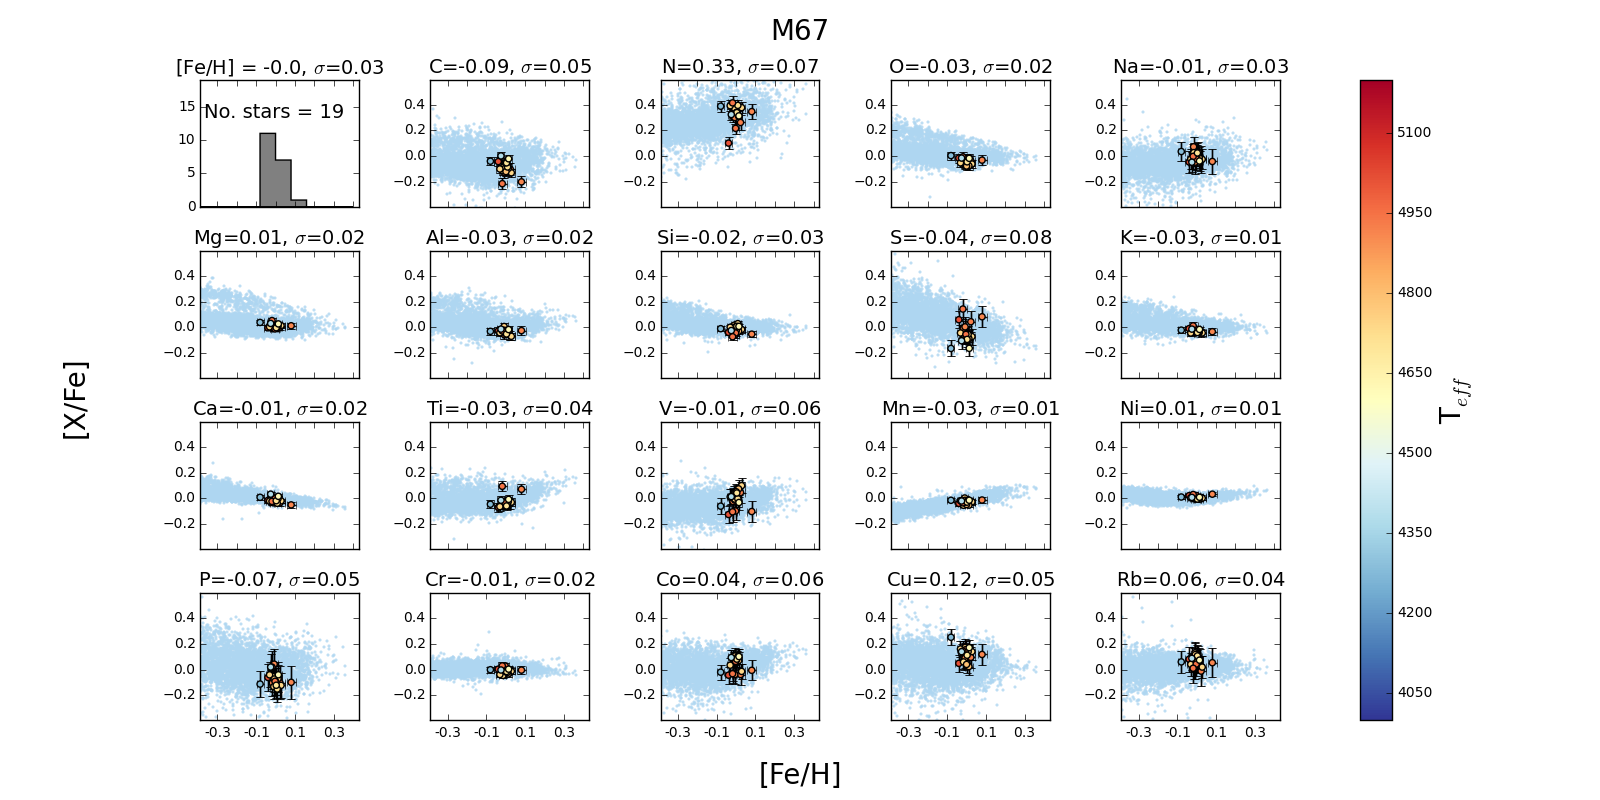
\includegraphics[scale=0.5]{/Users/ness/Dropbox/new_laptop/Apogee_elements/DR13/oldnorm/20elem7_tc2_nofilt.png}
    %      \includegraphics[scale=0.5]{/Users/ness/Dropbox/new_laptop/Apogee_elements/DR13/oldnorm/20elem7_tc2_nofilt.pdf}
               \includegraphics[scale=0.5]{20elem7_tc2_nofilt.pdf}
  \caption{ M67 stars with SNR = 438 $\pm$ 266 }
\label{fig:c1}
\end{figure*}

\begin{figure*}
\centering
   %     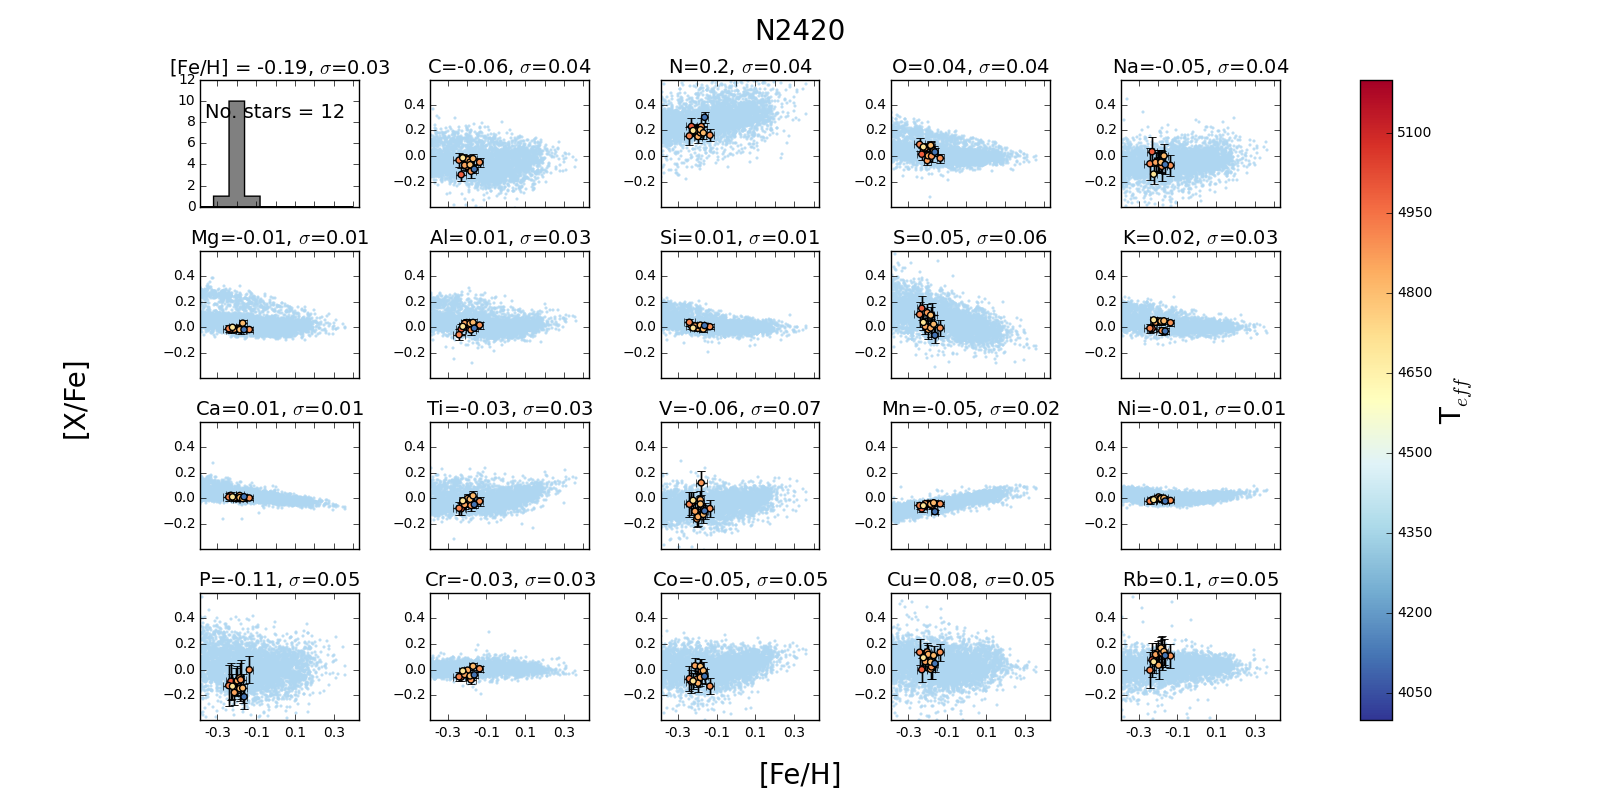
\includegraphics[scale=0.5]{/Users/ness/Dropbox/new_laptop/Apogee_elements/DR13/oldnorm/20elem12_tc2_nofilt.png}
 % \includegraphics[scale=0.5]{/Users/ness/Dropbox/new_laptop/Apogee_elements/DR13/oldnorm/20elem12_tc2_nofilt.pdf}   
  \includegraphics[scale=0.5]{20elem12_tc2_nofilt.pdf}  
  \caption{ NGC2420 stars with SNR = 311 $\pm$ 248 }
\label{fig:c2}
\end{figure*}

\begin{figure*}
\centering
      %  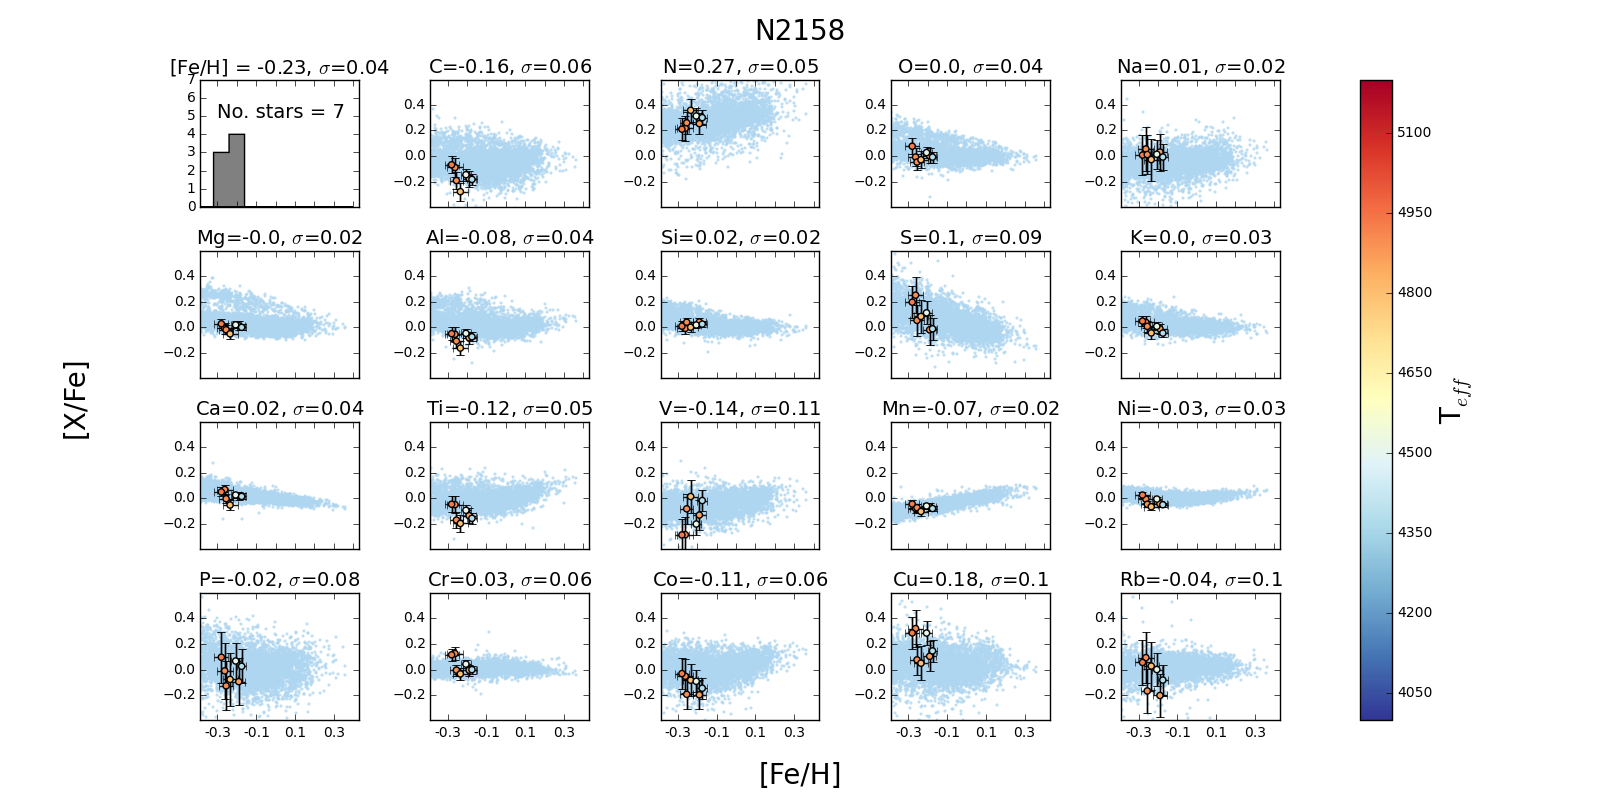
\includegraphics[scale=0.5]{/Users/ness/Dropbox/new_laptop/Apogee_elements/DR13/oldnorm/20elem11_tc2_nofilt.png}
           %    \includegraphics[scale=0.5]{/Users/ness/Dropbox/new_laptop/Apogee_elements/DR13/oldnorm/20elem11_tc2_nofilt.pdf}
                     \includegraphics[scale=0.5]{20elem11_tc2_nofilt.pdf}
  \caption{ NGC2158 stars with SNR = 96 $\pm$ 37 }
\label{fig:c3}
\end{figure*}

\begin{figure*}
\centering
        %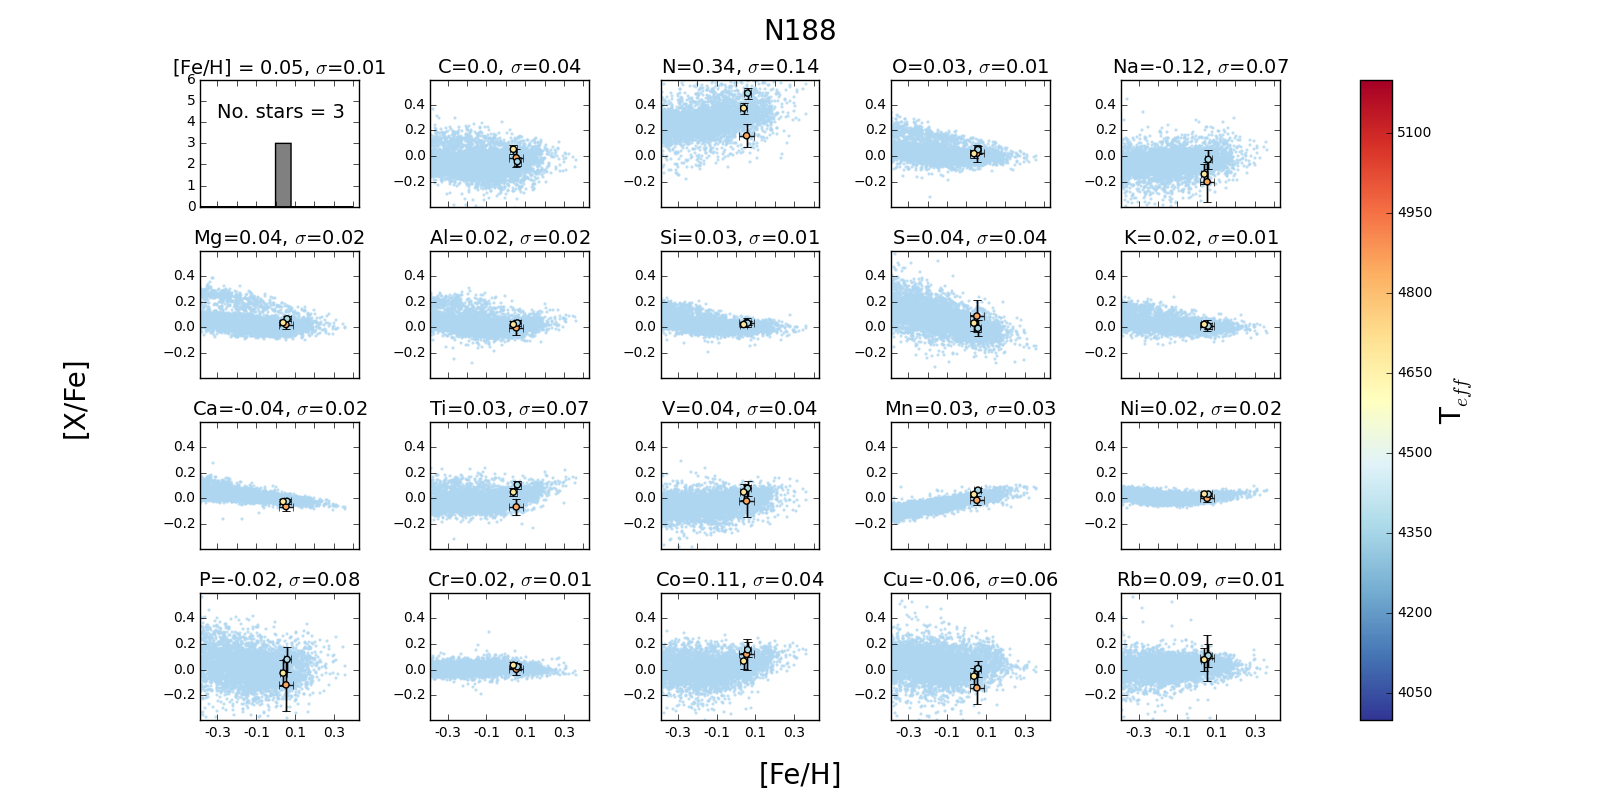
\includegraphics[scale=0.5]{/Users/ness/Dropbox/new_laptop/Apogee_elements/DR13/oldnorm/20elem10_tc2_nofilt.png}
       %       \includegraphics[scale=0.5]{/Users/ness/Dropbox/new_laptop/Apogee_elements/DR13/oldnorm/20elem10_tc2_nofilt.pdf}
                 \includegraphics[scale=0.5]{20elem10_tc2_nofilt.pdf}
  \caption{ NGC188 stars with SNR = 462 $\pm$ 381}
\label{fig:c4}
\end{figure*}

\begin{figure*}
\centering
        %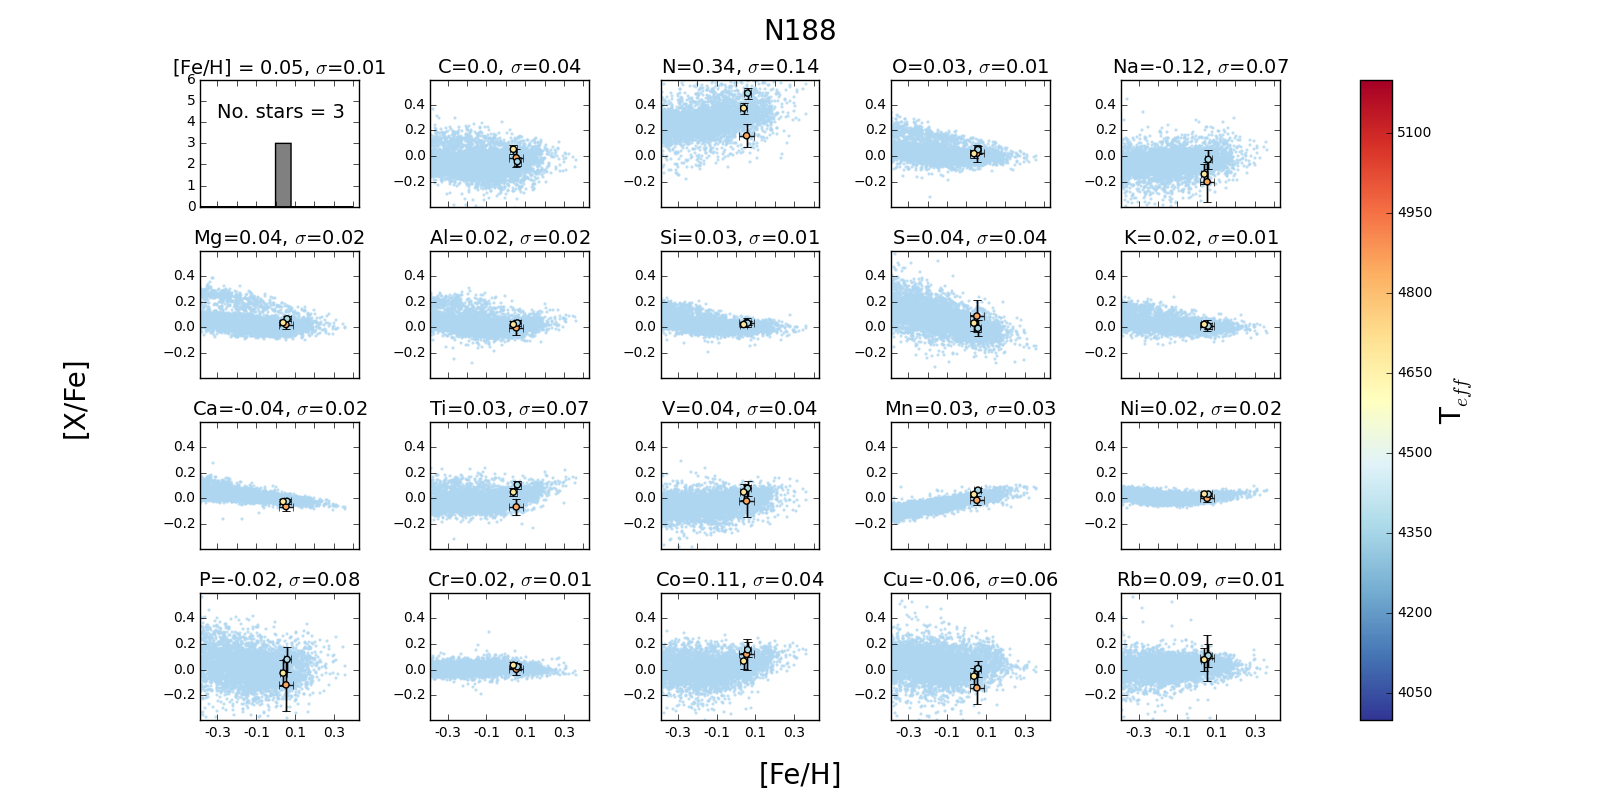
\includegraphics[scale=0.5]{/Users/ness/Dropbox/new_laptop/Apogee_elements/DR13/oldnorm/20elem10_tc2_nofilt.png}
         %     \includegraphics[scale=0.5]{/Users/ness/Dropbox/new_laptop/Apogee_elements/DR13/oldnorm/20elem8_tc2_nofilt.pdf}
           \includegraphics[scale=0.5]{20elem8_tc2_nofilt.pdf}
  \caption{ M71 stars with SNR = 249 $\pm$ 78}
\label{fig:c4}
\end{figure*}


\begin{figure*}
\centering
     %   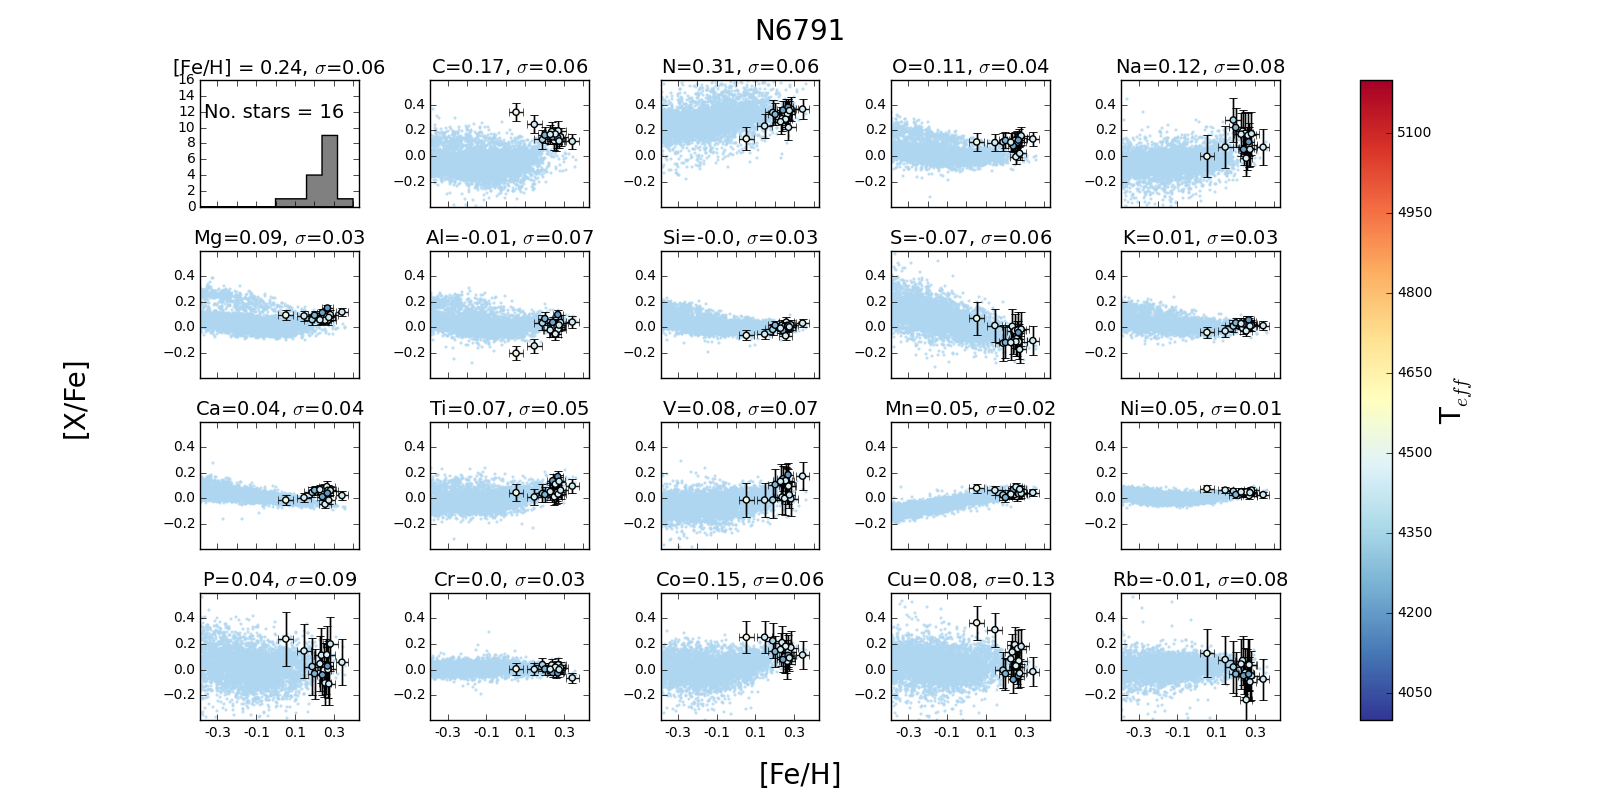
\includegraphics[scale=0.5]{/Users/ness/Dropbox/new_laptop/Apogee_elements/DR13/oldnorm/20elem-3_tc2_nofilt.png}
 %         \includegraphics[scale=0.5]{/Users/ness/Dropbox/new_laptop/Apogee_elements/DR13/oldnorm/20elem-3_tc2_nofilt.pdf}
    \includegraphics[scale=0.5]{20elem-3_tc2_nofilt.pdf}
  \caption{ NGC6791 stars with SNR = 159 $\pm$ 186 }
\label{fig:c5}
\end{figure*}

\begin{figure*}
\centering
      %  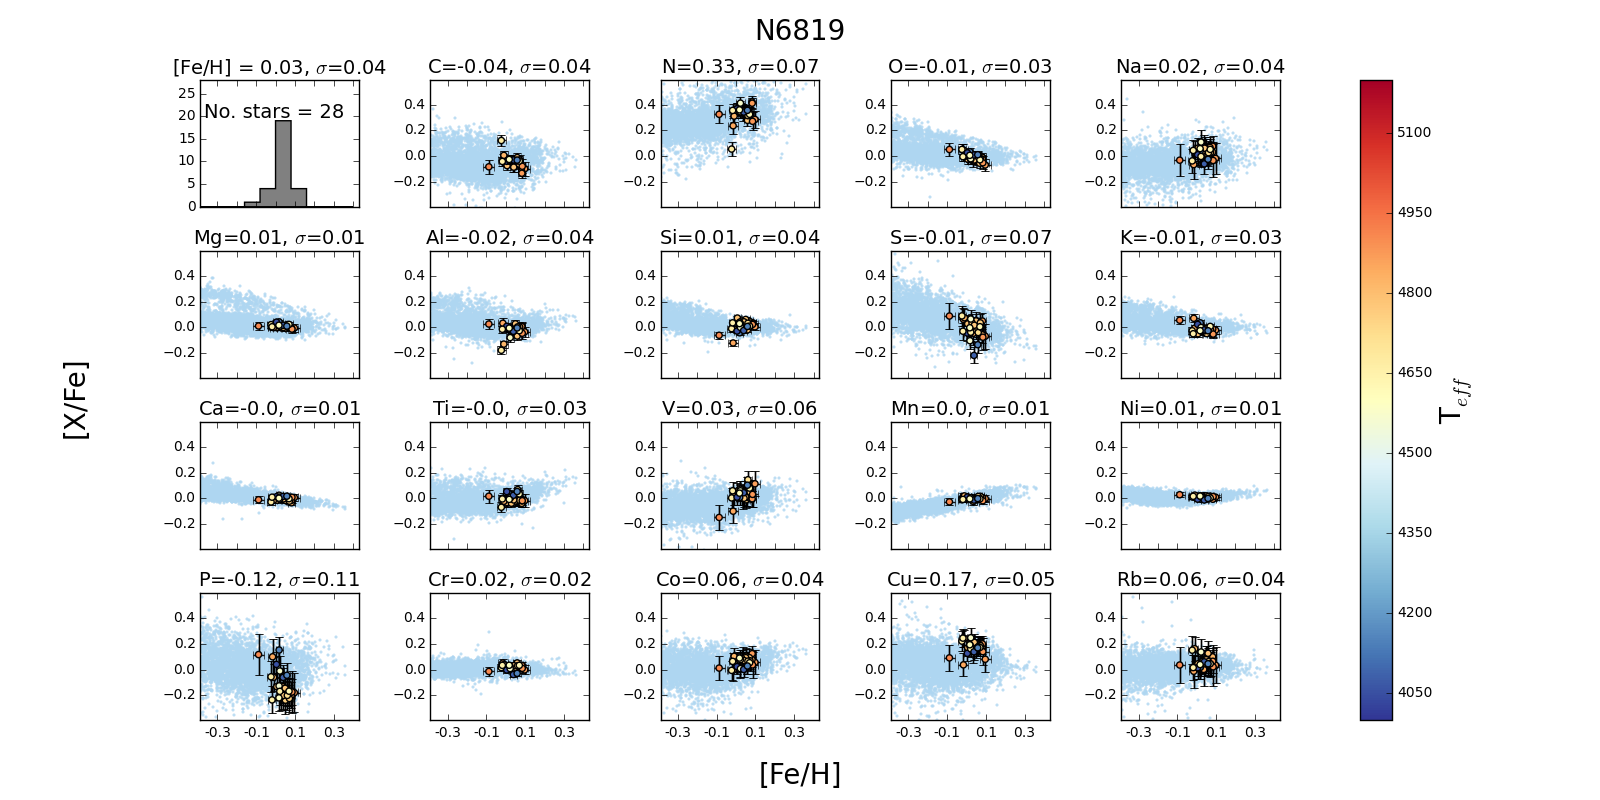
\includegraphics[scale=0.5]{/Users/ness/Dropbox/new_laptop/Apogee_elements/DR13/oldnorm/20elem-2_tc2_nofilt.png}
    %    \includegraphics[scale=0.5]{/Users/ness/Dropbox/new_laptop/Apogee_elements/DR13/oldnorm/20elem-2_tc2_nofilt.pdf}
        \includegraphics[scale=0.5]{20elem-2_tc2_nofilt.pdf}
  \caption{ NGC6819 stars with SNR = 303 $\pm$ 183 }
\label{fig:c6}
\end{figure*}

\begin{figure*}
\centering
%        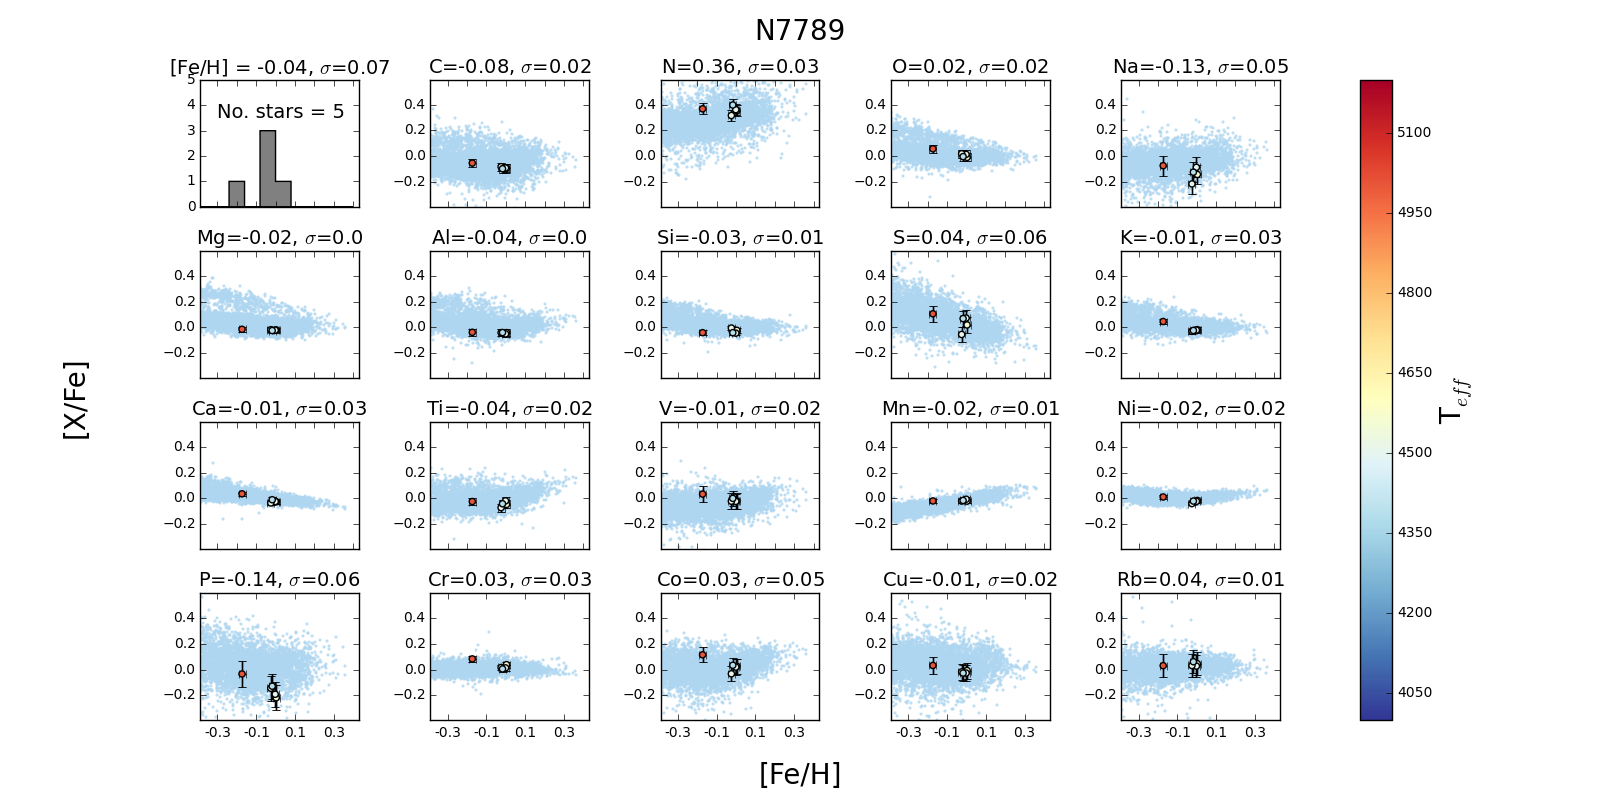
\includegraphics[scale=0.5]{/Users/ness/Dropbox/new_laptop/Apogee_elements/DR13/oldnorm/20elem-1_tc2_nofilt.png}
% \includegraphics[scale=0.5]{/Users/ness/Dropbox/new_laptop/Apogee_elements/DR13/oldnorm/20elem-1_tc2_nofilt.pdf}
  \includegraphics[scale=0.5]{20elem-1_tc2_nofilt.pdf}
  \caption{ NGC7789 stars with SNR = 657 $\pm$ 165 }
\label{fig:7n}
\end{figure*}



\section{Discussion}


Stars in open clusters are believed to be born from single star forming aggregates and therefore, thought to be chemically homogeneous \citep[e.g.][]{deSilva2007,deSilva2009}. Such chemical similarity of stars born together has been used to identify members of moving groups or co-natal groups in the Milky Way including using abundances alone \citep[e.g.][]{Majewski2012a, Hogg2016} as well as chemically exceptional groups of stars \citep[e.g.][]{Schiavon2016, Martell2016}.  Using APOGEE data and \aspcap\ abundances, \citet{Ting2016} placed a constraint on the initial cluster mass function for the old disk stars in the Milky Way.  Although many individual clusters have been studied in numerous studies, including using \apogee\ data \citep[e.g.][]{Souto2016, Cuhna2015, F2013} and the inter-cluster dispersion is demonstrated to be relatively small and on the order of measurement errors themselves, there has very little assessment in the literature as to the true intrinsic dispersion of clusters in their many elements other than Bovy et al., 2016 who was able to put firm and very small limits on the intrinsic inter-cluster dispersion, although without delivering individual abundance measurements, for 3 of the APOGEE clusters. 

While there has been some investigation of the statistical intra-cluster similarity \citep[][]{M2014, deSilva2015}, our aim to determine the intrinsic abundance dispersion of the \apogee\ clusters given our measurements and measurement errors and use the 7 calibration clusters to set the expectation for when stars in the \apogee\ sample are \textit{not} born together, in the same molecular cloud. This latter quantification in particular will be relevant for assessing the much larger sample of \apogee\ data and chemical dimensionality of the Milky Way disk. 

talk about precision not accuracy.... 

\subsection{Modeling the intrinsic Dispersion}

Our measured abundances within clusters are on the order of the precision we achieve in the quadratic sum of the cross-validation and formal measurement errors for the individual stars for each element. This indicates that our clusters are near homogeneous in their measured abundances. However, whether or not open clusters have any intrinsic spread in their abundances is critical for the pursuit of chemical tagging and understanding the formation of these systems (e.g. Bovy, Martin's latest paper 2nd author) so we wish to formally determine for each element, for each cluster, what the true mean and intrinsic dispersion is, given our data. 

To do this, we minimise the negative log likelihood of the following model, which represents the distribution of the elements within a cluster, for each element $i$, for $n$ stars, for the mean \textcolor{blue}{$\bar{x}$} and dispersion \textcolor{blue}{$\sigma_n$}. 

We also optimise over the sigma-clipping of the input data$ \delta x_{i, n}$ so that if there is an anomalous data point this may be excluded at the optimal solution to our model.  The sigma clipping is set at a minimum value of 1.5, however only in two cases of the 7 clusters for the 20 elements is the minimum reached at this clipping; on average the optimal sigma-clipping is $\approx$ 3: almost all stars are therefore included in the measurement of the intrinsic mean and dispersion.\\

$P({x_i} | \textcolor{blue}{\bar{x}, \sigma_x, i }) =  \prod_{n=1}^{N} \frac{1}{\sqrt{2 \pi (\delta x_{ \textcolor{blue}{i}, n} ^2 + \textcolor{blue}{{\sigma}_n^2}})} . e ^ - {\frac{\textcolor{blue}{(\bar{x}} - x_{\textcolor{blue}{i}, n})^2 }{2(\delta x_i^2 + \textcolor{blue}{\sigma_n^2)}}}$ \\

In this optimisation, the input data that we are summing over is the measurement for that element $i$ for every star, $x_n$  and the error on that measurement, $\delta x_n^2$, where for each element $i$, where we take $\delta x_n^2$ to be the quadrature error of the formal error on the star and the signal-to-noise dependent cross validation error for that element (measured using repeat observations of the \apogee\ calibration stars as shown in the Appendix). 

We find that for given this model, for each cluster, the intrinsic mean is very near to that of the measured mean assuming a Gaussian distribution for all stars. Furthermore the intrinsic dispersions for all element enhancements with respect to iron are zero, with the exception of Ni ($=$ 0.02 dex) in NGC2158, N ($\sigma_i$$=$ 0.13 dex) in N188 (although there are only 3 stars in this cluster and one anomalous measurement driving this, so this measurement is not robust on the basis of small sample size) and Mg ($\sigma_i$$=$ 0.01) in NGC6791. If our errors on these measurements are overestimated by up to 20\% however the small dispersions for Ni and Mg in NGC2158 and NGC6791 also become consistent with zero. We do find intrinsic dispersion in the \feh\ abundance for a number of the clusters, which persists even if we assume an error under-estimate of up to 20\%. We report an intrinsic dispersion in \feh\ of $\sigma_i$ $=$ 0.03 dex in NGC6819, $\sigma_i$$=$0.03 in NGC2158, $\sigma_i$$=$ 0.01 in M67,  $\sigma_i$$=$ 0.02 in NGC2420 and $\sigma_i$ = 0.01 in NGC6791. NGC2420, NGC7789 and NGC188 all have intrinsic iron dispersions consistent with  $\sigma_i$$=$0. These intrinsic dispersion measurements are consistent with the findings of Bovy for M67 and NGC2420 although our NGC6819 intrinsic dispersion is 0.01 larger than the upper limit Bovy (2016) places for the Fe measurement of this open cluster. 


\subsection{Absolute measurements}

We have demonstrated in Tables 1 and 2 that our absolute measurements, (by design) agree very well with those of \aspcap, only our dispersions are much smaller due to higher precision measurements with \tc. Comparing to the literature reveals a significant variation in the absolute values of measured abundances, which is a long standing and known problem in the community  (e.g. Slimanic et al., 2015 - see my old paper for correct spelling) that is now being addressed by placing different surveys directly on a common (APOGEE) scale (e.g. Ho et al., 2016, Casey et al., 2016). We are interested, for the purposed of chemical tagging and for assessing chemical similarity and dissimilarity of stars in general, only precision. We can make these chemical assessments within individual surveys with large numbers of stars, like APOGEE, RAVE and GALAH (cite all) or among surveys if they are placed directly on the same scale. 
Examining the literature on individual clusters, many have been studied by independent groups. NGC2420 has been studied by de Souto et al and we report vey similar dispersions to their careful by hand analysis. We compare well with their individual abundance measurements to the degree that the \aspcap
 results are similar (see their discussion). For NGC7789 our abusolute Mg measurement is low compared to all literature values by $\sim$ 0.1--0.2 dex although there is a very broad range in all measured abundances in the literature for this cluster (see Table 2 of \citet{Overbeek2015}). \\
 write one sentence about every cluster referencing some literature.\\

%Here we are using all wavelength region \tc\ is free to use correlations in order to determine abundance trends. We can also implement masking, using only the relevant lines and tests give very comparable results for the well-measured elements, some elements become marginally higher precision, some lower. Using masking does not work well for abundance labels which are coming in that are not as well measured by aspcap, namely  Na, Cu, P and Co - using masking for these elements leads to 50\% larger dispersion in the open clusters. We will discuss the merits of masking in Ness et al., in prep (2016). 

%Here we discuss each cluster
%Discuss that created distance, looked at max distance between all, conclude if great than, not born from same cloud


\subsection{Intra and Inter cluster similarity: nearest neighbour paris}

 %run -i makehistabund_general_oconly
 %nn_diff = chitest[unid]
 % nn_same = chitest[unid]
\begin{figure}[h!]
%\includegraphics[scale=0.2]{/Users/ness/new_laptop/Apogee_elements/DR13/oldnorm/chi2red.pdf} 
\includegraphics[scale=0.2]{chi2red.pdf} 
  \caption{reduced chi2 distribution of nearest neighbour pairs of stars within and between clusters. There are 52 pairs in the intra-cluster distribution and 58 in the inter-cluster distribution}
\label{fig:snr_error}
\end{figure}

Even stars from the same cluster can have very distant neighbours, the metric we can infer that if stars have chi2 > 2.8 they are not from a common birth site. 

Here show the nearest neighbour and that find new member of NGC188 in this way and reference paper in prep: was outside of the nominal radius of the open cluster. ID of one found this one. 



results with and without filters
- our aim is to get highest precision. achieved if the cannon can make use of all of the information: using all correlations; our aim is tagging and cross validation shows we reproduce - include filter version in the abstract
our precision for filters is XX times larger and about 30\% smaller than aspcap. Our open cluters are high snr and we preform comparably to aspcap at this snr. 


 exactly the same abundances - this is what is the challenge to tagging 
propose not inter but intra that limit tagging ability.
of clusters, the two are extremely simimalr. 
proceed to mapping abundance space similarity for metal-rich end of disk not find common orign but abundances alone; prospect for pairs. 

We find that the open clusters are very homogeneous, in their alpha, iron-peak and light elements that we measure. We are able to measure the 20 abundance of NGC, M67 and . Clusters are proxies for general birth sites and we want to understand just how homogenous these birth sites are: thus how similar two sibling stars are expected to be. 

 our aim is to set the calibration to assess the chemical dimensionality of the Milky Way:
%We use \tc\ to determine the precision with which we can measure chemical abundances of stars in the \apogee\ survey. We do this to pursue our aim of classifying stars that are most chemically similar and here use the open clusters to calibrate the precision we can measure as indicative of homogenous birth sites. To achieve our precision measurements, we have had to remove critical systematics, of abundance variation with the point spread function. 

%makegradientfilters_works_informationcriterion.py



\section{Conclusion}

By making modifications to \tc\ in order to cope with the variation in the abundance measurements input at training time on the LSF of each star we have been able to determine very precise abundances for 90 identified red giant members of the seven open clusters targeted in \apogee\ for the purpose of calibration. We report an intrinsic dispersion in all abundance measurements consistent with $\sigma=$ 0 except for \feh\ which has a spread in four of the clusters: $\sigma_i$=0.01, 0.02,  0.03, 0.03 in M67, NGC2420 NGC2158 and NGC6791 respectively. 
Fe of $\sigma_i$ $=$ 0.03 dex in NGC6819, $\sigma_i$$=$0.03 in NGC2158, $\sigma_i$$=$ 0.01 in M67,  $\sigma_i$$=$ 0.02 in NGC2420 and $\sigma_i$ = 0.01 in NGC6791. NGC2420, NGC7789 and NGC188 all have intrinsic iron dispersions consistent with  $\sigma_i$$=$0. 

\pagebreak

\section{Appendix}
%in /Users/ness/new_laptop/Apogee_elements/19labels/
%run -i makecompare_nofilt_dr13.py
%run -i snr_plot.py'
To do: Also show when implement the filtering on this Figure and discuss that much worse for some elements as coming in at training much worse:
Using a calibration set of data available as part of the public release of DR13, which included the co-added spectra and all individual visits, the precision of \tc\ was assessed as a function of signal to noise. Each data point in Figure \ref{fig:snr_error} was determined by measuring the dispersion of the difference between the high signal to noise and low signal to noise value of the labels for each of the 1000 stars in the calibration set. The Figure shows the dependence across SNR of 10 to 200, where the precision flattens above SNR of about 150. \tc\ and \aspcap\ compare well at high SNR but at low SNR \tc\ is more precise by a factor of 2-4 (also see Ness et al., 2015). In this comparison, \aspcap\ is restricted to the wavelength intervals for individual elements and show that can not perform well for the elements where aspcap can not perform well - use the unmasked version to get the highest precision for all the elements - can only get a subset of elements as training on imprecise labels. Learns correlations but clearly can reproduce the input at take 10 percent out cross validation so verified that if test data representatitve of training data this is good; any divergence can also be assessed by fit of data to model , including around individual elements. only used global chi2 in this paper but could image doing a chi2 around each element. 

%run -i snr_plot.py

\begin{figure*}[h!]
%\includegraphics[scale=0.45]{/Users/ness/new_laptop/Apogee_elements/19labels/snrplot.pdf} 
%\includegraphics[scale=0.45]{/Users/ness/new_laptop/Apogee_elements/19labels/rms_snr_both_dr132.pdf} 
\includegraphics[scale=0.45]{rms_snr_both_dr132.pdf} 
  \caption{SNR dependent performance for each label of \tc\ in red and \aspcap\ in black and with masking in blue - discuss this}
\label{fig:snr_error}
\end{figure*}

\bibliography{tc.bib}

\end{document}

\subsection{Training Data} 
We constructed a training set of data that spans the range of our test set of stars which are the open cluster red giants plus the \apogee\ red clump stars catalogued by Bovy et al., (2015). For our labels we used the DR13 corrected labels with small additional corrections for the LSF dependence (see section X). For high precision results, noisy training data must be excluded and we took care to construct a clean training set, with anomalous abundance measurements removed. We selected high SNR stars (SNR  $>$ 200) in our training set with abundance measurements which sit in physically plausible parameter space, e.g. the trends seen by Bensby et al., (20XX) and also the measurements of the high fidelity red clump sample used by Nidiver et al., 20XX. Additionally we excluded all stars with any bad flag set. as the parameter space for each element of the well measured red clump stars and which had no bad flags set. Our training data comprises 500 stars and spans the following range in stellar parameters:
\teff\ = 3715 $-$ 6079 K  \\
\logg\ = 0.80 $-$ 3.92 dex \\
\feh\ = --1.02 $-$ 0.32 dex \\
%\subsection{Test Data} 